%-*-latex-*-
\sectionthree{Infix notation}
\begin{python0}
from solutions import *; clear()
\end{python0}

The \lq\lq usual'' way of writing arithmetic expression
where a binary operator is placed in the middle is called
infix notation.
Here's an example
\[
\text{\texttt{1 + 2 * 3}}
\]
Now as mentioned earlier, you need parentheses
if you want to change the standard order of
evaluating as infix expression.
So any algorithm to evaluate infix expressions
must taken into account parentheses -- which is a pain.
For instance
\[
\text{\texttt{(1 + 2) * 3}}
\]

Of course you can do this:
make one scan of the string processing only
the highest order operators.
Then I redo that with the operators at the second
precedence level.
Etc.
For instance, say your algorithm can handle only \texttt{+,-,*,/}
then for the following you first do \texttt{*,/}
scanning the string once, and then you do
\texttt{+,-} scanning the resulting string a second time:
\texttt{
\begin{align*}
&  \hspace{0.521cm} \texttt{0 - 1 + 2 \underline{*} 3 - 4 / 5 * 6} \\
&= \texttt{0 - 1 + 6 - 4 \underline{/} 5 * 6} \\
&= \texttt{0 - 1 + 6 - 0 \underline{*} 6} \\
&= \texttt{0 \underline{-} 1 + 6 - 0} \\
&= \texttt{-1 \underline{+} 6 - 0} \\
&= \texttt{5 \underline{-} 0} \\
&= \texttt{5} 
\end{align*}
}
(The underline denotes my finger running across the string
left-to-right and stopping when I see an operator that I should
evaluate.)



\begin{ex}
Implement the above idea.
What is the runtime in terms of the length of the string?
(Assume that all integers are 1-digit in length.)
Assume that the string is given as a queue (the left end is the front
of the queue).
What data structures do you need?
\qed
\end{ex}

But let's see if we can do better ...

The general idea is actually pretty simple.
For now, I'll use the idea below to compute arithmetic expressions.
Later on, we'll see that it can be used to build \lq\lq trees".

Suppose you look at 
\[
\text{\texttt{1 + 2 * 3}}
\]
How would you evaluate it as a program?
How do you decide that \texttt{+} should come after \texttt{*}?
Of course as you process the character left to right, you can't see 
\texttt{*} yet if you're processing \texttt{+} or even when you're
processing \texttt{2}.
You would then have to remember \texttt{1 + 2}
and when you process \texttt{*}, you know that you cannot process
\texttt{1 + 2} because \texttt{2} should be used by \texttt{*}:
$2$ \textit{belongs} to \texttt{*}.
So we have to keep \texttt{1 + 2} somewhere.

Now suppose we know that we need to process \texttt{2 * 3} first.
(This is due to historical conventions -- we do multiplications
before additions.)
What does that mean?
We have to remember \texttt{1 + 2}, but don't execute the addition.
We then have to take the \texttt{2} out of what we remembered
for executing \verb!2 * 3!.
That means that we're taking the \textit{last} thing out of our
memory device.
Right?
The \texttt{1} went in first, then the \texttt{+} and then the \texttt{2} --
\verb!2! was the \textit{last} thing we have to remember.

See that?

We have to take \verb!2! out of the things we stash somewhere
(the \verb!1! and the \verb!+! and the \verb!2!)
and then we took the \verb!2! out.
Again this is important: \verb!2! was the last thing we have to remember
and \verb!2! is the thing we have to take out from our stash.


AHA! ... We probably need a stack!

In the above case, how do we know that \texttt{*} can go?

Because there's no more operators to compete against it.
And why must \texttt{+} wait for \texttt{*}?
Because \texttt{*} has a higher precedence.
To make it easy to read, I'm going to write
\[
\texttt{* > +}
\]
to say that \texttt{*} has higher precedence.
Now why is there no one else to compete again \texttt{*}?
Because it's the last operator -- there's no operator after it.
Note that this can happen in a different way too ...
look at
\[
\texttt{1 + 2 * 3 * 4}
\]
The first \texttt{*}, i.e.,
\[
\texttt{1 + 2 \underline{*} 3 * 4}
\]
\textit{beat} the second \texttt{*}
\[
\texttt{1 + 2 * 3 \underline{*} 4}
\]
because they are at the \textit{same} precedence level ... and
\texttt{*} is \defone{left-to-right associative}
i.e.,
\[
\texttt{1 * 2 * 3} 
\]
means
\[
\texttt{(1 * 2) * 3}
\]
This behavior of \verb!*! is also called \defone{left associative}.

So the first \texttt{*} beats the second.
Remember this!

But what if I have
\[
\texttt{1 + 2 * 3 + 4}
\]
and I'm now about to process the second \texttt{+}:
\[
\texttt{1 + 2 * 3 \underline{+} 4}
\]
The subexpression
\[
\texttt{1 + 2 * 3}
\]
is not processed yet.
Why? Because the \texttt{*} beats the \texttt{+} so \texttt{+}
has to wait.
But I also cannot let \texttt{*} go ahead since
the next operator might beat \texttt{*}.
Now when I read the \texttt{+} in
\[
\texttt{1 + 2 * 3 \underline{+} 4}
\]
I know now that \texttt{*} can go ahead.
This gives me
\[
\texttt{1 + 6 \underline{+} 4}
\]
But wait! ... Since \texttt{+} is left-to-right associative,
this means that
the first \texttt{+} also go ahead too so that I get this:
\[
\texttt{7 \underline{+} 4}
\]
So when do I stop in the general case?
From the above example, it's clear that I keep going until
I see an operator with precedence order strictly less than the \texttt{+}
that I just read.
Correct?
Remember this!

So ... hmmm ... what if we have this:
\[
\text{\texttt{1 * 2 \underline{+} 3}}
\]
Suppose we've read \texttt{1 * 2} and stored them somewhere
(but it's not evaluvated yet ... we're
waiting to see if the next operator should go first)
and I'm about to the \texttt{+}.
Then once we see the \texttt{+}, since \texttt{*} beats \texttt{+},
\[
\texttt{* > +}
\]
we know that \texttt{*} can go first.
So we pull \texttt{1 * 2} out of our memory so as to evaluate it.
That gives me \texttt{2}.
Now I have to do the \texttt{+}, i.e.., I have to process 
\texttt{2 + 3}.

In order to use previous processing rules, I will first put the 
\texttt{2} (due to the evaluation of \texttt{1 * 2})
back into my memory device.
This will make the process uniform.
For instance with \texttt{2} in the memory device, after processing
\texttt{+ 3}, I will have \texttt{2 + 3} in the memory device.
Only when I see that there's no more input for processing then 
I know that no other operator is beating \texttt{+} and therefore
I can compute \texttt{2 + 3}.

Wait wait wait ... that means that when I look at the \texttt{+},
I need to recall the \texttt{1 * 2} from a container but
the important value is \texttt{*}.
So if I store \texttt{1 * 2} in a stack, the \texttt{*} is \textit{not}
at the
top. Sure, I can pop \texttt{2} off and then I will see the \texttt{*}.

AHA! ... So ...

For me to see the \texttt{*} quickly,
I can keep the operators in a separate memory device.
So I think I'll have \textit{two} memory devices:
one for the integers and one for the operators.

What about something like 
\[
\text{\texttt{1 + 2 + 3}}
\]
In that case, once I've remember \texttt{1 + 2},
when I see the next \texttt{+} I know that \texttt{+} remembered
can go ahead since they are the same precedence level
and \texttt{+} associates left to right.
Right?

OK.
We now have enough information to do a complete
trace using the above ideas.
\begin{enumerate}[nosep]
  \li We continually read the data from the input. The input
  is made up of integers and operators.
  \li For memory, we have two stacks, the first
  for remembering
  integers (call it \texttt{intstack}) and second for operators
  (call it \texttt{opstack}).
  \li When I read an integer, I push it onto \texttt{intstack}.
  \li When I read an operator \texttt{op}, I do the following:
  \begin{enumerate}[nosep]
    \li If \texttt{op} $>$ top of \texttt{opstack}:
    I push \texttt{op} onto \texttt{opstack}.
    \li If \texttt{op} $\leq$ top of \texttt{opstack}:
    I pop an operator off \texttt{opstack} and use it to
    evaluate the top two values on \texttt{intstack}, pushing
    the result back onto \texttt{intstack}.
    I keep doing this until \texttt{op} $>$ the top of
    \texttt{opstack}.
    After that I push \texttt{op} onto \texttt{opstack}.
  \end{enumerate}
  \li When there's no more input to read, I continually
  pop an operator off \texttt{opstack} and evaluate
  two values from the top of \texttt{intstack}, pushing the
  result back onto \texttt{intstack}.
  The final result is on the top of \texttt{intstack}.
\end{enumerate}
Clearly the two cases of processing the \texttt{op} can be combined.
So I get this:
\begin{enumerate}[nosep]
  \li We continually read the data from the input. The input
  is made up of integers and operators.
  \li For memory, we have two stacks, the first
  for remembering
  integers (call it \texttt{intstack}) and second for operators
  (call it \texttt{opstack}).
  \li When I read an integer, I push it onto \texttt{intstack}.
  \li When I read an operator \texttt{op}, I do the following:
  \begin{enumerate}[nosep]
    \li As long as \texttt{op} $\leq$ top of \texttt{opstack}:
    I pop an operator off \texttt{opstack} and use it to
    evaluate the top two values on \texttt{intstack}, pushing
    the result back onto \texttt{intstack}.
    \li After that, I push \texttt{op} onto \texttt{opstack}.  
  \end{enumerate}
  \li When there's no more input to read, I continually
  pop an operator off \texttt{opstack} and evaluate
  two values from the top of \texttt{intstack}, pushing the
  result back onto \texttt{intstack}.
  The final result is on the top of \texttt{intstack}.
\end{enumerate}

(You see that there's a lot of \lq\lq operate on the
top two values on the stack and put the result back onto the top''.
See the next section for \textbf{stack machines}.)

There are some optimizations:
For instance on evaluating with an operator on the
\texttt{opstack},
note that I pop two values off the \texttt{intstack},
operator on them, push the result back onto \texttt{intstack}.
I keep doing this.
So it's better \textit{not} to push the result back onto the
stack since it will be popped off again in the next around.
You push the result only when the loop has ended.
So the above becomes this:
\begin{enumerate}[nosep]
  \li We continually read the data from the input. The input
  is made up of integers and operators.
  \li For memory, we have two stacks, the first
  for remembering
  integers (call it \texttt{intstack}) and second for operators
  (call it \texttt{opstack}).
  \li When I read an integer, I push it onto \texttt{intstack}.
  \li When I read an operator \texttt{op}, I do the following:
  \begin{enumerate}[nosep]
    \li If \texttt{op} $\leq$ top of \texttt{opstack}:
    \begin{enumerate}[nosep]
      \li I pop off an integer from the \texttt{intstack} and store it
      in \texttt{a}
      \li As long as \texttt{op} $\leq$ top of \texttt{opstack}:
      I pop an operator off \texttt{opstack},
      pop off an integer from the \texttt{intstack}
      and store it in \texttt{b}.
      I compute \texttt{(b op a)} and store it in \texttt{a}.
      \li I push \texttt{a} onto \texttt{intstack}
    \end{enumerate}
    \li After that, I push \texttt{op} onto \texttt{opstack}.  
  \end{enumerate}
  \li When there's no input, I do the following:
  If \texttt{opstack} is empty,
  I return the top of \texttt{intstack}.
  Otherwise I do the following:
  \begin{enumerate}[nosep]
    \li I pop an integer off \texttt{intstack} and store in \texttt{a}.
    \li As long as \texttt{opstack} is not empty, I do the following:
    I pop an operator off \texttt{opstack} and store in \texttt{op},
    I pop an integer off \texttt{intstack} and store in \texttt{b},
    I compute \texttt{(b op a)} and store in \texttt{a}.
    \li Otherwise, I pop an integer off the top of \texttt{intstack}
    and store in \texttt{a}.
    (If there are more than two values in \texttt{intstack}, there's an
    error.)
  \end{enumerate}
\end{enumerate}



Once we're comfortable with the ideas, we'll write down the
algorithm.
Let's forget about the parentheses for now and 
try an example using what we have discovered.
Let's look at this:
\[
\texttt{0 - 1 + 2 * 3 - 4 / 5 * 6}
\]
You would expect the evaluation to be like this:
\[
\texttt{((0 - 1) + (2 * 3)) - ((4 / 5) * 6)}
\]
Here we go!

{\scriptsize
\begin{console}
              intstack opstack (top on left)
                              PROCESS INPUT
0-1+2*3-4/5*6 []       []
                              0:Push intstack
 -1+2*3-4/5*6 [0]      []
                              -:Push opstack
  1+2*3-4/5*6 [0]      [-]
                              1:Push intstack
   +2*3-4/5*6 [0,1]    [-]
                              +:+ <= -. Compute with top of
                                opstack until opstack empty or
                                + > top.
                                Then push + onto opstack.
   +2*3-4/5*6 [-1]     []
   +2*3-4/5*6 [-1]     [-]
    2*3-4/5*6 [-1]     [+]
                              2:Push intstack
     *3-4/5*6 [-1,2]   [+]
                              *:* > +. Push opstack
      3-4/5*6 [-1,2]   [+,*]
                              3:Push intstack
       -4/5*6 [-1,2,3] [+,*]
                              -:- <= *. Compute with top of
                                opstack until opstack empty or
                                - > top.
                                Then push - onto opstack
        4/5*6 [-1,6]   [+]
        4/5*6 [5]      []
        4/5*6 [5]      [-]
                              4:Push intstack
         /5*6 [5,4]    [-]
                              /:/ > -. Push opstack
          5*6 [5,4]    [-,/]
                              5:Push intstack
           *6 [5,4,5]  [-,/]  
                              *:* <= /. Compute with top of
                                opstack until opstack empty or
                                * > top.
                                Then push * onto opstack
            6 [5,4,5]  [-,/]  
            6 [5,0]    [-]
                              6:Push intstack
              [5,0,6]  [-,*]  
                              NO MORE INPUT: Compute with
                              top of opstack until opstack
                              empty                             
              [5,0]    [-]
              [5]      []
\end{console}
}
You can see the computations with this:
\[
\text{\texttt{\underline{\underline{\underline{0 - 1} + \underline{ 2 * 3}} -
      \underline{\underline{4 / 5} * 6}}}}
\]
The algorithm at this point look like this:
\begin{console}
ALGORITHM: EVALUATE-INFIX (without parentheses)
INPUT: x = list/string of integers and operators

intstack is a stack of integers
opstack is a stack of operators

while there is still data in x:
    take data out of x
    if data taken out of x is an int:
        push that int onto intstack
    otherwise (i.e., data is an operator)
        call the data op
        if opstack is not empty and op <= top of opstack:
            let a = pop intstack
            while opstack is not empty and
                op <= top of opstack:
                let b = pop intstack
                let op1 = pop opstack
                let a = (b op1 a)
            push a onto intstack
        push op onto opstack

if opstack is empty:
    return top of intstack
else:
    let a = pop intstack
    while opstack is not empty:
        let b = pop intstack
        let op1 = pop opstack
        let a = (b op1 a)
    return a
\end{console}
In the above, when I write \lq\lq \texttt{(b op1 a)}''
I mean evaluate the operator \texttt{op1} with values
\texttt{b} and \texttt{a}.
For instance is \texttt{op1} is \texttt{-}
and \texttt{a} and \texttt{b} are \texttt{2} and \texttt{7}
respectively, then \texttt{(b op a)} is \texttt{(7 - 2)}
i.e., \texttt{5}.

You can add pseudocode to return error codes.
For instance just before
returning, the stack should have exactly one
value -- you can check for that.
Also, remember that since all operators considered here
are binary, you need two integers on the stack to
evaluate the operator.
You can check for that; if you don't have two integers,
then again you can return an error code.

One very important observation is this:
Although \texttt{*} and \verb!/! has to go first
  because they have higher precedence order,
  note that in the above the leftmost subtraction \texttt{-}
  actually gets evaluated first.
  But this is OK since the end result is the same.
  So this algorithm obeys operator precedence rules
  \textit{and} it evaluates as soon as it is possible.
  If you look at the above picture:
\[
\text{
  \texttt{
    \underline{\underline{\underline{0 - 1} + \underline{2 * 3}} -
      \underline{\underline{4 / 5} * 6}}
  }
}
\]
you'll see that the subtract on the left will not \lq\lq disturb''
the multiplication in the middle.
I haven't talked about trees yet, but if you look at this expression
tree, you should be able to guess what's happening:

\begin{center}

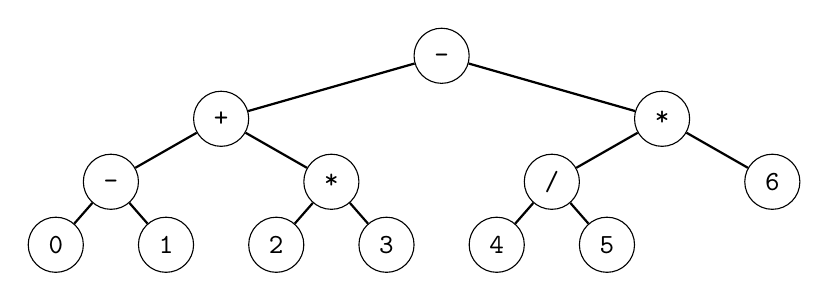
\begin{tikzpicture}
\node at (4.8999999999999995,-0.8) [circle,draw,minimum size=7mm] (A) {\texttt{-}};
\node at (2.0999999999999996,-1.6) [circle,draw,minimum size=7mm] (B) {\texttt{+}};
\node at (7.699999999999999,-1.6) [circle,draw,minimum size=7mm] (C) {\texttt{*}};
\node at (0.7,-2.4000000000000004) [circle,draw,minimum size=7mm] (D) {\texttt{-}};
\node at (3.5,-2.4000000000000004) [circle,draw,minimum size=7mm] (E) {\texttt{*}};
\node at (6.3,-2.4000000000000004) [circle,draw,minimum size=7mm] (F) {\texttt{/}};
\node at (9.1,-2.4000000000000004) [circle,draw,minimum size=7mm] (G) {\texttt{6}};
\node at (0.0,-3.2) [circle,draw,minimum size=7mm] (H) {\texttt{0}};
\node at (1.4,-3.2) [circle,draw,minimum size=7mm] (I) {\texttt{1}};
\node at (2.8,-3.2) [circle,draw,minimum size=7mm] (J) {\texttt{2}};
\node at (4.199999999999999,-3.2) [circle,draw,minimum size=7mm] (K) {\texttt{3}};
\node at (5.6,-3.2) [circle,draw,minimum size=7mm] (L) {\texttt{4}};
\node at (7.0,-3.2) [circle,draw,minimum size=7mm] (M) {\texttt{5}};
\draw [-,thick] (A) -- (B);
\draw [-,thick] (A) -- (C);
\draw [-,thick] (B) -- (D);
\draw [-,thick] (B) -- (E);
\draw [-,thick] (C) -- (F);
\draw [-,thick] (C) -- (G);
\draw [-,thick] (D) -- (H);
\draw [-,thick] (D) -- (I);
\draw [-,thick] (E) -- (J);
\draw [-,thick] (E) -- (K);
\draw [-,thick] (F) -- (L);
\draw [-,thick] (F) -- (M);

;
\end{tikzpicture}
    
\end{center}


Think of computation with this tree as \lq\lq bottom to top''.
You'll notice that the subtree corresponding to the subtraction on
the left and multiplication in the middle (of the original expression)
are in different subtrees that do not disturb each other.
So although \texttt{*} should go before the leftmost \texttt{-},
the result would be unchanged if I do the leftmost \texttt{-} first.
And why is \lq\lq evaluate as soon as possible'' a good thing?

Because this means that your containers will remove contents
sooner and therefore you save on space.

\begin{ex}
Here's another important observation:
Do you notice that in the above trace, the operators on the operator stack
is always in decreasing precedence order as you go from the top of the stack to the bottom?
Is this always true?
\qed
\end{ex}

\begin{ex}
Using the ideas from above (and after studying the trace above),
now trace the following yourself:
\[
\text{\texttt{1 - 5 * 3 / 2 + 1 + 2 * 3 \% 4}}
\]
What is the maximum stack size?
(Try a few more until you are familiar with the algorithm.)
\qed
\end{ex}

Next let's handle \texttt{(} and \texttt{)}.
What should we do if we see
\[
\text{\texttt{1 * (2 + 3)}}
\]
Say I have processed \texttt{1 *}.
What should happen to them?
Of course there's no evaluation: I remember these two
pieces of data, the integer in one stack and the multiplication
in another.
Now, when I see the left parenthesis:
\[
\text{\texttt{1 * \underline{(}2 + 3)}}
\]
if you do this by hand, you wouldn't do any computation.
The left parenthesis is just to force us to work on this
subexpression:
\[
\text{\texttt{1 * \underline{(2 + 3)}}}
\]
Now ... this does mean that in some sense the \texttt{(}
\textit{blocks} us from processing \texttt{1 *}.
So ... if we put the \texttt{(} onto the stack of operators,
all we need to do is to make sure our algorithm does not let us past
\texttt{(}, except when we see a \texttt{)}.
When you look at previous ideas, all we need to do is to make sure that
\texttt{+,-,*,/,\%} have higher precedence than \texttt{(}.

And what do we do when we see \texttt{)}?
That means that the subexpressions enclosed by this \texttt{)}
(and the matching \texttt{(} that started this subexpression)
must be completely evaluated.

To be concrete consider this:
\[
\text{\texttt{1 + (2 + 3 * 4 - 5) / 6}}
\]
Say we have read the data up to this point:
\[
\text{\texttt{1 + \underline{(}2 + 3 * 4 - 5) / 6}}
\]
On reading \texttt{(}, I will push it onto my operator stack.
Then I proceed using previous ideas so that \texttt{2} is
pushed onto the integer stack.
Now when I read the \texttt{+}:
\[
\text{\texttt{1 + (2 \underline{+} 3 * 4 - 5) / 6}}
\]
since I impose the rule that \texttt{(} has lower precedence,
\texttt{(} will stay on the stack; \texttt{+} is pushed onto the
operator, waiting to see if it beats the next operator.

After \texttt{3} is pushed onto the integer stack, I read \texttt{*}:
\[
\text{\texttt{1 + (2 + 3 \underline{*} 4 - 5) / 6}}
\]
\texttt{*} beats \texttt{+} (on the top of the operator stack).
So \texttt{*} is pushed onto the operator stack and waits to
see if it beats the next operator.
After \texttt{4} is pushed onto the integer stack, I see \texttt{-}:
\[
\text{\texttt{1 + (2 + 3 * 4 \underline{-} 5) / 6}}
\]
Ahhh ... at this point \texttt{*} on top of the operator stack
beats \texttt{-}, so multiplication goes ahead and using \texttt{3}
and \texttt{4} on the integer stack with \texttt{*}, I get \texttt{12}
which is pushed back onto the integer stack.
At this point the operator stack contains
\[
\text{\texttt{[+, (, +]}}
\]
(top of the stack is on the right) and the integer stack contains
\[
\text{\texttt{[1, 2, 12]}}
\]
But \texttt{-} is \texttt{<= +} the top of the operator stack
(and they are both left-to-right associative).
So \texttt{+} gets to go ahead.
Which means that the operator stack becomes
\[
\text{\texttt{[+, (]}}
\]
and the integer stack becomes
\[
\text{\texttt{[1, 14]}}
\]
At this point, since \verb!( < -!, I push \verb!-! onto the
operator stack.
\texttt{5} is then read and stored on the integer stack:
\[
\text{\texttt{1 + (2 + 3 * 4 - \underline{5}) / 6}}
\]
And now ... here's where things get interesting.
I read the \texttt{)}:
\[
\text{\texttt{1 + (2 + 3 * 4 - 5\underline{)} / 6}}
\]
I now operate on all the operators on the operator stack
\textit{until I see a matching } \texttt{(}.
The operator stack looks like this:
\[
\text{\texttt{[+, (, -]}}
\]
(don't forget that the multiplication and addition has already gone ahead
and are evaluated)
and the integer stack looks like this:
\[
\text{\texttt{[1, 14, 5]}}
\]
(The \texttt{14} comes from \texttt{2 + 3 * 4}.)
This means that I will be performing \texttt{14 - 5} (to get \texttt{9}).
After that, I see \texttt{(} on the stack.
I stop the operations, throw away the \texttt{(}.
I do \textit{not} push the \texttt{)} onto the stack.
At this point the original subexpression \texttt{(2 + 3 * 4 - 5)}
is evaluated (to get \texttt{9}) and is placed on the stack.
In other words the integer stack looks like this:
\[
\text{\texttt{[1, 9]}}
\]
and the operator stack looks like this:
\[
\text{\texttt{[+]}}
\]
Get it?

Now you might be worried about this point ...
I said that once I see \texttt{)}, it signals that it's
time to completely finish the subexpression.
Then I said to work through all the operators on the stack
until I see the first \texttt{(} to appear on the top of the
operator stack.
Notice that I don't check for precedence --
I simply go through the operators on the operator
stack one at a time until I see \texttt{(}.
Why don't I worry about the precedence order in this case?
Because ... after the \texttt{(}, remember that
if I see an operator with strictly higher precedence I push,
and if I see one that is lower or equal precedence, I evaluate the opereator
that is already on the top of the stack.
Think about this:

That means that
the operators after \texttt{(} all the way to the top of the stack
must be in ascending precedence order!!!!
For instance if I'm reading the following the expression
at \verb!)!:
\[
\text{\texttt{1 + (2 + 3 * 4\underline{)} + 5}}
\]
the operator stack looks like this:
\[
\text{\texttt{[+, (, +, *]}}
\]
It's impossible to have this scenario for your operator stack
when you hit a \verb!)!:
\[
\text{\texttt{[+, (, *, -]}}
\]
and it's also impossible to have this:
\[
\text{\texttt{[+, (, +, -]}}
\]
It's also possible to have this:
\[
\text{\texttt{[+, (, +, *, (, +, /, (, -, \%]}}
\]
i.e., from the \texttt{(} up to (but not including) the next \texttt{(},
the precedence order increases.
Again, the operator from the \texttt{(} to the top
(or up the next \texttt{(} but not including it)
must be in ascending precedence order:
\begin{align*}
&\text{\texttt{[+, \underline{(, +, *}, (, +, /, (, -, \%]}} \\
&\text{\texttt{[+, (, +, *, \underline{(, +, /}, (, -, \%]}}
\end{align*}


So when I evaluate starting at the top of the operator
stack down to \texttt{(}, I am going from high to low precedence order.
That's why I don't have to check for precedence order for this scenario.
Get it?

Here's a trace:

{\scriptsize
\begin{console}
                  intstack opstack (top on left)
                                           PROCESS INPUT
0-(1+2+3*(4-5)+6) []         []
                                           0:Push intstack
 -(1+2+3*(4-5)+6) [0]        []
                                           -:Push opstack
  (1+2+3*(4-5)+6) [0]        [-]
                                           (:Push opstack
   1+2+3*(4-5)+6) [0]        [-,(]
                                           1:Push intstack
    +2+3*(4-5)+6) [0,1]      [-,(]
                                           +:+ > (. Push opstack
     2+3*(4-5)+6) [0,1]      [-,(,+] 
                                           2:Push intstack
      +3*(4-5)+6) [0,1,2]    [-,(,+] 
                                           +:+ <= +. Compute with top of
                                             opstack until opstack empty or
                                             + > top.
                                             Then push + onto opstack.
       3*(4-5)+6) [0,3]      [-,(]
       3*(4-5)+6) [0,3]      [-,(,+]
                                           3:Push intstack
        *(4-5)+6) [0,3,3]    [-,(,+]
                                           *:* > +. Push opstack
         (4-5)+6) [0,3,3]    [-,(,+,*]
                                           (:Push opstack
          4-5)+6) [0,3,3]    [-,(,+,*,(]
                                           4:Push intstack
           -5)+6) [0,3,3,4]  [-,(,+,*,(]  
                                           -:- > (. Push opstack
            5)+6) [0,3,3,4]  [-,(,+,*,(,-]
                                           5:Push intstack
             )+6) [0,3,3,4,5][-,(,+,*,(,-]
                                           ):Compute with top of opstack
                                             until (.
              +6) [0,3,3,-1][-,(,+,*,(]
              +6) [0,3,3,-1][-,(,+,*]
                                          +:+ <= *. Compute with top of
                                            opstack until opstack empty or
                                            + > top.
                                            Then push + onto opstack.      
               6) [0,3,-3]  [-,(,+]
               6) [0,0]     [-,(]
               6) [0,0]     [-,(,+]
               6) [0,0]     [-,(,+]
                                          6:Push intstack
                ) [0,0,6]   [-,(,+]
                                          ):Compute with top of opstack
                                             until (.
                  [0,6]     [-,(]
                  [0,6]     [-]
                                          NO MORE INPUT: Compute with
                                          top of opstack until opstack
                                          empty
                  [-6]      []
\end{console}
}

\begin{console}
ALGORITHM: EVALUATE-INFIX (with parentheses)
INPUT: x = list/string of integers and operators

intstack is a stack of integers
opstack is a stack of operators

while there is still data in x:
    take data out of x
    if data taken out of x is an int:
        push that int onto intstack
    otherwise (i.e., data is an operator)
        call the data op
        if op is '(':
            push op onto opstack
        elif op is ')':
            let a = pop intstack
            while top of opstack is not '(':
                let b = pop intstack
                let op1 = pop opstack
                let a = (b op1 a)
            push a onto intstack
        otherwise:
            if opstack is not empty and op <= top of opstack:
                let a = pop intstack
                while opstack is not empty and
                    op <= top of opstack:
                    let b = pop intstack
                    let op1 = pop opstack
                    let a = (b op1 a)
                push a onto intstack
            push op onto opstack

if opstack is empty:
    return top of intstack
else:
    let a = pop intstack
    while opstack is not empty:
        let b = pop intstack
        let op1 = pop opstack
        let a = (b op1 a)
    return a
\end{console}

\begin{ex}
What if you do this:
Ensure that all subexpressions
are parenthesized -- include the largest one.
So if you need to evaluate \texttt{1 + 2 * 3},
evaluates this instead:
\texttt{(1 + 2 * 3)}.
How will that change your pseudocode?
\qed
\end{ex}

\begin{ex}
Write a \cpp\ function that accepts an infix expression
described by a \verb!std::vector! of strings
and perform infix evaluation on the expression.
For instance
when you execute this
\begin{console}
// 0-(1+2+3*(4-5)+6)
std::vector< std::string> > e;
e.push_back("0");
e.push_back("-");
e.push_back("(");
e.push_back("1");
e.push_back("+");
e.push_back("2");
e.push_back("3");
e.push_back("*");
e.push_back("4");
e.push_back("-");
e.push_back("5");
e.push_back(")");
e.push_back("+");
e.push_back("6");
int x = eval_infix(s, true);
\end{console}
The integer value of \verb!-6! is given to \texttt{x} and
the following output is shown below.
(If the last parameter is set to \texttt{false} then \verb!eval_infix()!
will not print any output.)
{\small
\begin{Verbatim}[frame=single]
0-(1+2+3*(4-5)+6) []          []
 -(1+2+3*(4-5)+6) [0]         []
  (1+2+3*(4-5)+6) [0]         [-]
   1+2+3*(4-5)+6) [0]         [-,(]
    +2+3*(4-5)+6) [0,1]       [-,(]
     2+3*(4-5)+6) [0,1]       [-,(,+] 
      +3*(4-5)+6) [0,1,2]     [-,(,+] 
       3*(4-5)+6) [0,3]       [-,(]
       3*(4-5)+6) [0,3]       [-,(,+]
        *(4-5)+6) [0,3,3]     [-,(,+]
         (4-5)+6) [0,3,3]     [-,(,+,*]
          4-5)+6) [0,3,3]     [-,(,+,*,(]
           -5)+6) [0,3,3,4]   [-,(,+,*,(]  
            5)+6) [0,3,3,4]   [-,(,+,*,(,-]
             )+6) [0,3,3,4,5] [-,(,+,*,(,-]
              +6) [0,3,3,-1]  [-,(,+,*,(]
              +6) [0,3,3,-1]  [-,(,+,*]
               6) [0,3,-3]    [-,(,+]
               6) [0,0]       [-,(]
               6) [0,0]       [-,(,+]
               6) [0,0]       [-,(,+]
                ) [0,0,6]     [-,(,+]
                  [0,6]       [-,(]
                  [0,6]       [-]
                  [-6]        []
\end{Verbatim}
}
[Put the output into array of strings and then figure out the maximum column width
that you need when everything is done. \textit{Then} you perform the printing.]
\qed
\end{ex}
  

\begin{ex}
Using the ideas from above (and after studying the trace above),
now trace the following yourself:
\[
\text{\texttt{1 - 5 * (3 / 2) + ((1 + (2 * 3) \% 4)}}
\]
Try a few more until you're comfortable with the algorithm.
\qed
\end{ex}



\begin{ex}
  Think about this very carefully:
  all the operators in the above examples are left-to-right associative,
  i.e. left associative. For instance $1 + 2 + 3 + 4$ means
  $((1 + 2) + 3) + 4$.
  This is the same for subtraction, integer division, and integer mod.
  What if an operator is right associative?
  Suppose you also want to handle exponentiation.
  Say we use the character \verb!^! to denote exponentiation.
  For instance \verb!2 ^ 3! is \verb!8!.
  Recall that \verb!^! is right-to-left associative, i.e.,
  right associative.
  In other words
  \verb!2 ^ 3 ^ 4 ^ 5!
  is \verb!2 ^ (3 ^ (4 ^ 5))!.
  This is different from \verb!+! which is left-to-right associative:
  \verb!2 + 3 + 4!
  is \verb!(2 + 3) + 4)!.
\qed
\end{ex}

  
\begin{ex}
  The above examples are binary operators.
  What about unary operators?
  You know that \verb!+! can be either a binary operator
  or a unary operator.
  The unary \verb!+! is the \lq\lq positive of" operator.
  To avoid this ambiguity, let's talk about the factorial.
  How about adding the factorial to the above algorithm?
  For instance \texttt{3!} is \texttt{6}.
  Note that it's unary.
  Of course
  \texttt{3!!!} is \texttt{((3!)!)!}.
  After you are done think about this:
  \verb@!@ is written on the \textit{right} of the argument.
  The
  \lq\lq positive of" \verb!+!
  and
  \lq\lq negative of" \verb!-!
  is written on the \textit{left} of the argument.
  How does the computation of \verb!++++3!
  differ from \verb@3!!!!@?
\qed
\end{ex}

